%%%%%%%%% JPS abstract %%%%%%%%%%%%%%%%%%%%%%%%%%%%%%%%%%%%%%%%%%
\documentclass[12pt,a4paper]{jsarticle}

%%%%%%%%% packages %%%%%%%%%%%%%%%%%%%%%%%%%%%%%%%%%%%%%%%%%%%%%%
\usepackage[dvipdfmx]{graphicx} % Include figure files
\usepackage[%                           % 余白の設定
% mag=1400,%                              jarticle の場合(14ptに)
dvipdfm,truedimen,%
top=30truemm,bottom=20truemm,%
left=20truemm,right=20truemm]{geometry}
\usepackage{enumitem}
\usepackage{xurl}
\usepackage{amsmath,amssymb} % 数式環境
\usepackage{bm} % bold math
\usepackage[
  backend=biber,
  style=phys,
  articletitle=true,
  biblabel=brackets,
  sorting=none
]{biblatex}
\addbibresource{reference.bib}
\pagestyle{empty}

%%%%%%%%% header %%%%%%%%%%%%%%%%%%%%%%%%%%%%%%%%%%%%%%%%%%%%%%%%
\begin{document}
\vspace{-5pt}
\begin{center}
{\gt \Large 先行研究の日本語タイトル\cite{G_ng_r_2021} }\\[14pt]

{\gt \large 福島大理工 おなまえ}\\[5pt]

\end{center}

\vspace{10pt}
%%%%%%%%% main %%%%%%%%%%%%%%%%%%%%%%%%%%%%%%%%%%%%%%%%%%%%%%%%%%

\begin{abstract}
    本論文では…(背景・手法・結果を 200字程度でまとめる)
\end{abstract}

\section{研究背景}
\begin{description}[leftmargin=*]
    \item[分野の状況] 研究分野の現状を,歴史的経緯などを含め簡潔に文章でまとめる.
    \item[分野の課題](紹介する研究に対する)先行研究を整理し,これまで何が課題とされてきたのかを文章でまとめる.
    \item[研究の目的] 本研究の目的は何かを文章でまとめる.
    \item[新規性] これまでの研究と何が違うのかを文章でまとめる.
    \item[期待される効果] この研究によってもたらされる効果に関して文章でまとめる(研究の意義)
\end{description}
図の例
\begin{figure}[htbp]
    \centering
    \label{fig:research_goal}
    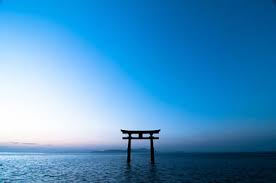
\includegraphics[width=0.5\linewidth]{./fig_1.png}
    \caption[転載元サイト]{\url{https://www.nta.co.jp/media/tripa/articles/gHvD8}より転載}
\end{figure}

\section{理論(手法)の概要}
\begin{enumerate}[leftmargin=*]
  \item 作用:$S = \frac{1}{2} \int d^4 x \sqrt{-g} \left( R + 2\Lambda + \mathcal{L}_m \right)$
  \item 各項がもたらす物理的な影響など
  \item 解析手法など
  \item 数値解析の対象となる式,初期条件など
\end{enumerate}

\section{主な結果と考察}
\begin{itemize}[leftmargin=*]
  \item 数値解析結果の物理的意味に関する結果と考察に関してまとめる
\end{itemize}

\section{結論と展望}
\begin{description}[leftmargin=*]
  \item[結論] 本研究によって示されたことをまとめる.
  \item[展望] 今後の研究に関して,どのようなことを考えているかをまとめる.
\end{description}

\section{メモ}
\begin{description}
    \item[自身の研究とのつながり] 研究の背景や目的を考える上で,どのような点が参考になったかをまとめる.
    \item[わからなかったこと] 論文を読み進めるうえで,わからなかったことをまとめる.
    \item[専門用語] 論文中に出てきた日本語訳の難しいと感じた専門用語をまとめる.
\end{description}

%%%%%%%%%%%%%%%%%%%%%%%%%%%% Figure 1 %%%%%%%%%%%%%%%%%%%%%%%%%%%%%%%%%%%%%
% \begin{figure}[h]
% \begin{center}
% \includegraphics[width=5cm]{JPS.eps}
% \end{center}
% \caption{日本物理学会のマーク.カラー図面が掲載できるようになった. }
% \end{figure}
%%%%%%%%%%%%%%%%%%%%%%%%%%%%%%%%%%%%%%%%%%%%%%%%%%%%%%%%%%%%%%%%%%%%%%%%%%%

\printbibliography[title=参考文献]

\end{document}
